\documentclass[tikz]{standalone}
\usepackage[english]{babel}
\usepackage[T1]{fontenc}
\usepackage[utf8]{inputenc}
\usepackage[absolute,overlay]{textpos}
\usepackage{graphicx}
\usepackage[export]{adjustbox}
\usepackage{svg}
\usepackage{IEEEtrantools}
\usepackage{physics,dsfont,mathrsfs,cancel,tensor,slashed,mathtools}

\usepackage{amsmath}
\usepackage{amsfonts}
\usepackage{bm}
\usepackage{setspace}
\usepackage{subcaption}
\usepackage{mwe}

\usepackage{tikz}
\usetikzlibrary{calc,patterns,decorations.pathmorphing,decorations.markings}
\usetikzlibrary{arrows.meta}
\usepackage{tikzscale}

% ----------------------------
% need this for spiral spring
\newcommand\spiral{} % just for safety
\def\spiral[#1](#2)(#3:#4)(#5:#6)[#7]{% \spiral[draw options](placement)(start angle:end angle)(start radius:final radius)[revolutions]
    \pgfmathsetmacro{\domain}{#4+#7*360}
    \pgfmathsetmacro{\growth}{180*(#6-#5)/(pi*(\domain-#3))}
    \draw [#1,
           shift={(#2)},
           domain=#3*pi/180:\domain*pi/180,
           variable=\t,
           smooth,
           samples=int(\domain/5)] plot ({\t r}: {#5+\growth*\t-\growth*#3*pi/180})
}

% ----------------------------
% need this for yield curve
% Définition des nouvelles options xmin, xmax, ymin, ymax
% Valeurs par défaut : -3, 3, -3, 3
\tikzset{
xmin/.store in=\xmin, xmin/.default=-3, xmin=-3,
xmax/.store in=\xmax, xmax/.default=3, xmax=3,
ymin/.store in=\ymin, ymin/.default=-3, ymin=-3,
ymax/.store in=\ymax, ymax/.default=3, ymax=3,
}
% Commande qui trace la grille entre (xmin,ymin) et (xmax,ymax)
\newcommand {\grille}
{\draw[help lines] (\xmin,\ymin) grid (\xmax,\ymax);}
% Commande \axes
\newcommand {\axes} {
\draw [>=stealth,->] (\xmin,0) -- (\xmax,0);
\draw [>=stealth,->] (0,\ymin) -- (0,\ymax);
}
% Commande qui limite l’affichage à (xmin,ymin) et (xmax,ymax)
\newcommand {\fenetre}
{\clip (\xmin,\ymin) rectangle (\xmax,\ymax);}
% ----------------------------

\begin{document}
%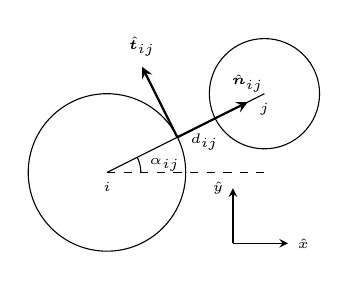
\begin{tikzpicture}
	\draw (0,0) circle(1) node[below] {\tiny$i$};
	\draw (2,1) circle(0.7) node[below] {\tiny$j$};
	\draw (0,0)--(2,1) node[pos=0.62, below] {\tiny$d_{ij}$};
	\draw[->,>=stealth, thick] (0.894,0.447)--(0.894+2/5^0.5,0.447+1/5^0.5) node[above] {\tiny$\hat{\bm n}_{ij}$};
	\draw[->,>=stealth, thick] (0.894,0.447)--(0.894-1/5^0.5,0.447+2/5^0.5) node[above] {\tiny$\hat{\bm t}_{ij}$};
    \draw[dashed] (0,0)--(2,0);
    \draw (0.43,0) arc(0:26.6:0.43) node[midway, right] {\tiny$\alpha_{ij}$};
    \draw [>=stealth, ->] (1.6, -0.9) -- (2.3, -0.9);
    \draw [>=stealth, ->] (1.6, -0.9) -- (1.6, -0.2);
    \draw (2.3, -0.9) node[right] {\tiny$\hat x$};
    \draw (1.6, -0.2) node[left] {\tiny$\hat y$};
\end{tikzpicture}

%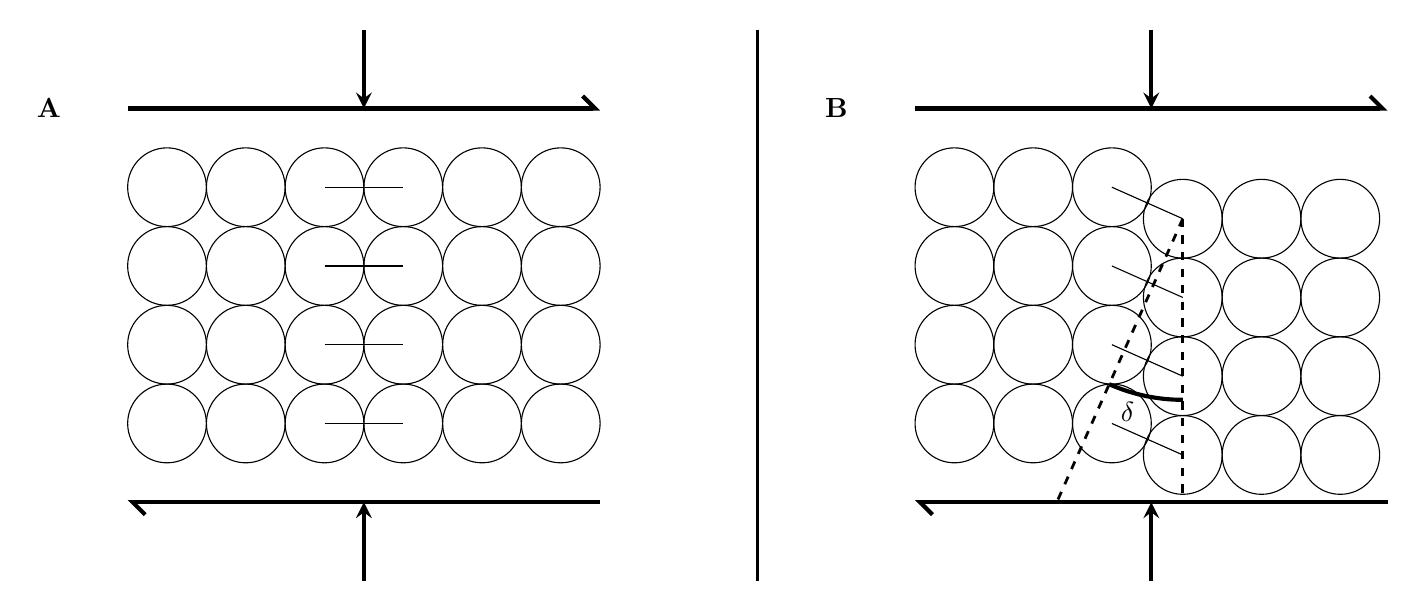
\begin{tikzpicture}
    \draw (-11.5,4) node {\textbf{A}};
    \draw (-1.5,4) node {\textbf{B}};

    \def \b {-10};
    \def \c {0.4};
    \def \d {0.1};
    \def \r {2.3};

    %circles

    \foreach \x in {0, 1, ..., 5}
        \foreach \y in {0, 1, ..., 3}
            \draw (\x + \b, \y) circle (0.5);

    \foreach \x in {0, 1, ..., 2}
        \foreach \y in {0, 1, ..., 3}        
            \draw (\x, \y) circle (0.5);

    \foreach \x in {3, 4, ..., 5}
        \foreach \y in {0, 1, ..., 3}        
            \draw (\x - \d, \y - \c) circle (0.5);

    % connections

    \foreach \y in {0, 1, ..., 3}   
        \draw (2 + \b,\y) -- (3 + \b,\y);

    \foreach \y in {0, 1, ..., 3}  
        \draw (2,\y) -- (3 - \d,\y - \c);

    % over/under lines

    \draw [line width = 1.5pt, >={Straight Barb[left]}, <-] (-0.5 + \b,-1) -- (5.5 + \b,-1);
    \draw [line width = 1.5pt, >={Straight Barb[left]}, ->] (-0.5 + \b,4) -- (5.5 + \b,4);

    \draw [line width = 1.5pt, >={Straight Barb[left]}, <-] (-0.5,-1) -- (5.5,-1);
    \draw [line width = 1.5pt, >={Straight Barb[left]}, ->] (-0.5,4) -- (5.5,4);

    % arrows

    \draw [line width = 1.5pt, >=stealth, ->] (2.5 + \b,5) -- (2.5 + \b,4);
    \draw [line width = 1.5pt, >=stealth, ->] (2.5 + \b,-2) -- (2.5 + \b,-1);

    \draw [line width = 1.5pt, >=stealth, ->] (2.5,5) -- (2.5,4);
    \draw [line width = 1.5pt, >=stealth, ->] (2.5,-2) -- (2.5,-1);

    % separation line

    \draw [line width = 1pt] (-2.5,5) -- (-2.5,-2);

    % angle

    \draw [line width = 1pt, dashed] (3 - \d, 3 - \c) -- (3 - \d, -1);
    \draw [line width = 1pt, dashed] (3 - \d, 3 - \c) -- ({3 - \d - (4*\c-\c*\c)/(1-\d)}, -1);
    \draw [line width = 1.5pt] (3 - \d,3 - \c - \r) arc (270:246:\r);
    \draw (\r - \d,0.15) node {$\delta$};


\end{tikzpicture}


%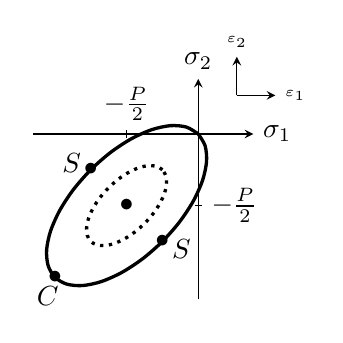
\begin{tikzpicture}[xmin=-3,xmax=1,ymin=-3,ymax=1,scale=0.70]
    \axes
    \draw [>=stealth, ->] (0.7, 0.7) -- (1.4, 0.7);
    \draw [>=stealth, ->] (0.7, 0.7) -- (0.7, 1.4);
    \draw [line width=1.2pt] [domain=0:2*pi,scale=0.65] plot[smooth] ({-2+2*cos(\x r)-sin(\x r)},{-2+sin(\x r)+2*cos(\x r)});
    \draw [line width=1.2pt,dotted] [domain=0:2*pi,scale=0.65] plot[smooth] ({-2+cos(\x r)-1/2*sin(\x r)},{-2+1/2*sin(\x r)+cos(\x r)});
    \draw [scale=0.65] (-2,-2) node {$\bullet$};
    \draw [scale=0.65] (-4,-4) node {$\bullet$};
    \draw [scale=0.65] (-3,-1) node {$\bullet$};
    \draw [scale=0.65] (-1,-3) node {$\bullet$};
    \draw [scale=0.65] (-4.2,-4) node[below] {$C$};
    \draw [scale=0.65] (-3,-0.8) node[left] {$S$};
    \draw [scale=0.65] (-1,-3.2) node[right] {$S$};
    \draw [scale=0.65] (-0.1,-2) -- (0.1,-2) node[right] {$-\frac{P}{2}$};
    \draw [scale=0.65] (-2,-0.1) -- (-2,0.1) node[above] {$-\frac{P}{2}$};
    \draw (1,0) node[right] {$\sigma_1$};
    \draw (0,1) node[above] {$\sigma_2$};
    \draw (1.4, 0.7) node[right] {\tiny$\varepsilon_1$};
    \draw (0.7, 1.4) node[above] {\tiny$\varepsilon_2$};
\end{tikzpicture}


%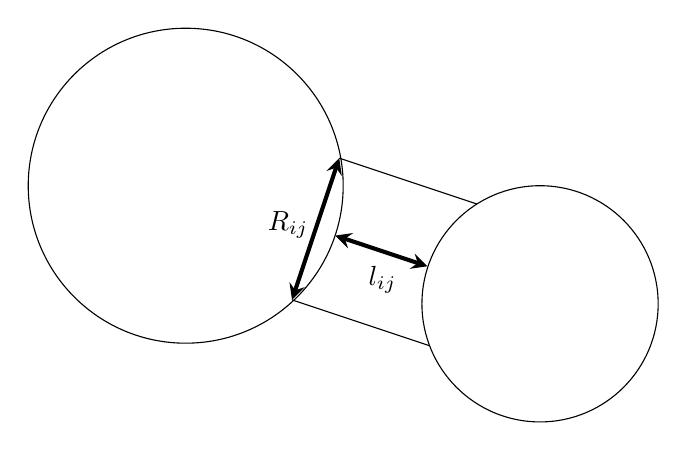
\begin{tikzpicture}

    \draw (0,0) circle(2);
    \draw (4.5,-1.5) circle(1.5);
    
    \draw [domain=1.95:3.7] plot(\x,-\x/3+1);
    \draw [line width = 1.5pt, >=stealth, <->] [domain=1.9:3.07] plot(\x,-\x/3);
    \draw [line width = 1.5pt, >=stealth, <->] [domain=1.35:1.95] plot(\x,3*\x-5.5);
    \draw [domain=1.35:3.1] plot(\x,-\x/3-1);
    
    \draw (1.3, -0.5) node {$R_{ij}$};
    \draw (2.5, -1.2) node {$l_{ij}$};

\end{tikzpicture}

%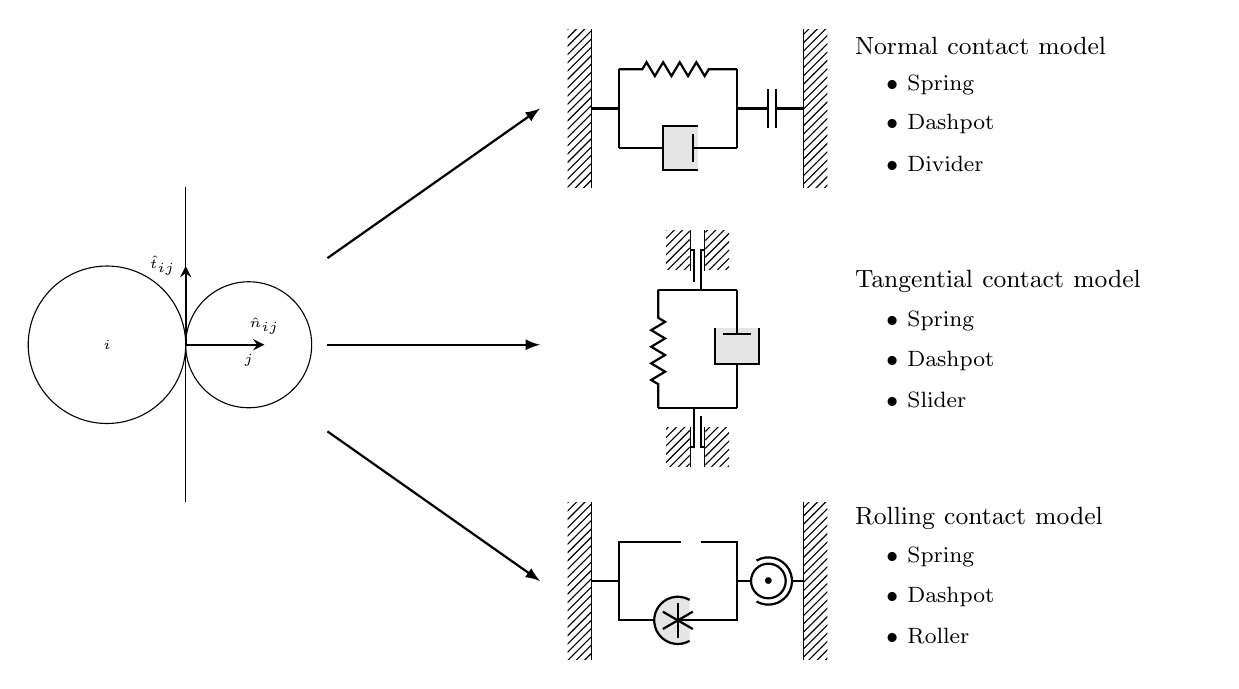
\begin{tikzpicture}
    \tikzstyle{spring}=[thick,decorate,decoration={zigzag,pre length=0.3cm,post length=0.3cm,segment length=6}]
    \tikzstyle{damper}=[thick,decoration={markings,  
      mark connection node=dmp,
      mark=at position 0.5 with 
      {
        \node (dmp) [thick,inner sep=0pt,transform shape,rotate=-90,minimum width=15pt,minimum height=10pt,draw=none] {};
        \filldraw [black!10,thick] ($(dmp.north east)+(2pt,0)$) -- (dmp.south east) -- (dmp.south west) -- ($(dmp.north west)+(2pt,0)$);
        \draw [thick] ($(dmp.north east)+(2pt,0)$) -- (dmp.south east) -- (dmp.south west) -- ($(dmp.north west)+(2pt,0)$);
        \draw [thick] ($(dmp.north)+(0,-5pt)$) -- ($(dmp.north)+(0,5pt)$);
      }
    }, decorate]
    \tikzstyle{ground}=[fill,pattern=north east lines,draw=none,minimum width=0.75cm,minimum height=0.3cm]

    %\draw [help lines] (-5,-3) grid (5,3);

    \begin{scope}[xshift=-7cm]
        \draw (-4,0) circle(1) node {\tiny$i$};
        \draw (-2.2,0) circle(0.8) node[below] {\tiny$j$};
        \draw (-3,-2) -- (-3, 2);
        \draw [thick, ->,>=stealth] (-3,0) -- (-3, 1) node[left] {\tiny$\hat t_{ij}$};
        \draw [thick, ->,>=stealth] (-3,0) -- (-2, 0) node[above] {\tiny$\hat n_{ij}$};

        \draw [thick, ->,>=latex] (-1.2,1.1) -- (1.5, 3);
        \draw [thick, ->,>=latex] (-1.2,0) -- (1.5, 0);
        \draw [thick, ->,>=latex] (-1.2,-1.1) -- (1.5, -3);
    \end{scope}

    \begin{scope}[xshift=0.5cm, yshift=0.8cm]
        \draw (0,3) node[text width=4cm,align=left] {\small Normal contact model};
        \draw (0,0) node[text width=4cm,align=left] {\small Tangential contact model};
        \draw (0,-3) node[text width=4cm,align=left] {\small Rolling contact model};

        \draw (0.4,2.5) node[text width=4cm,align=left] {\footnotesize $\bullet$ Spring};
        \draw (0.4,2) node[text width=4cm,align=left] {\footnotesize $\bullet$ Dashpot};
        \draw (0.4,1.5) node[text width=4cm,align=left] {\footnotesize $\bullet$ Divider};

        \draw (0.4,-0.5) node[text width=4cm,align=left] {\footnotesize $\bullet$ Spring};
        \draw (0.4,-1) node[text width=4cm,align=left] {\footnotesize $\bullet$ Dashpot};
        \draw (0.4,-1.5) node[text width=4cm,align=left] {\footnotesize $\bullet$ Slider};

        \draw (0.4,-3.5) node[text width=4cm,align=left] {\footnotesize $\bullet$ Spring};
        \draw (0.4,-4) node[text width=4cm,align=left] {\footnotesize $\bullet$ Dashpot};
        \draw (0.4,-4.5) node[text width=4cm,align=left] {\footnotesize $\bullet$ Roller};
    \end{scope}

    \begin{scope}[xshift=-2cm,yshift=3cm]
        \node (wall) [ground, rotate=-90, minimum width=2cm,yshift=-3cm] {};
        \draw (wall.north east) -- (wall.north west);
        
        \node (wall1) [ground, rotate=90, minimum width=2cm,yshift=0cm] {};
        \draw (wall1.north east) -- (wall1.north west);

        \draw [thick] (wall.90) -- (-2.5,0) -- (-2.5, 0.5);
        \draw [spring] (-2.5, 0.5) -- (-1,0.5);
        \draw [thick] (-1,0.5) -- (-1,0) -| (-0.6,0.25);
        \draw [thick] (-0.5,0.25) |- (wall1.90);

        \draw [thick] (wall.90) -- (-2.5,0) -- (-2.5, -0.5);
        \draw [damper] (-2.5, -0.5) -- (-1,-0.5);
        \draw [thick] (-1,-0.5) -- (-1,0) -| (-0.6,-0.25);
        \draw [thick] (-0.5,-0.25) |- (wall1.90);
    \end{scope}
    
    \begin{scope}[xshift=-3.5cm, yshift=1.7cm]
        \node (wall) [ground, rotate=-90, minimum width=0.5cm,xshift=3cm, yshift=-0.25cm] {};
        \draw (wall.north east) -- (wall.north west);
        
        \node (wall1) [ground, rotate=90, minimum width=0.5cm,xshift=-0.5cm,yshift=-0.25cm] {};
        \draw (wall1.north east) -- (wall1.north west);

        \node (wall2) [ground, rotate=90, minimum width=0.5cm,yshift=-0.25cm, xshift=-3cm] {};
        \draw (wall2.north east) -- (wall2.north west);

        \node (wall3) [ground, rotate=-90, minimum width=0.5cm,xshift=0.5cm,yshift=-0.25cm] {};
        \draw (wall3.north east) -- (wall3.north west);

        \draw [thick, rotate=90] (wall.90) |- (-2.5,0.04) -- (-2.5, 0.5);
        \draw [spring, rotate=90] (-2.5, 0.5) -- (-1,0.5);
        \draw [thick, rotate=90] (-1,0.5) -- (-1,-0.04);
        \draw [thick, rotate=90] (-0.9,0.04) -| (wall3.90);

        \draw [thick, rotate=90] (wall2.90) |- (-2.6,-0.04);
        \draw [thick, rotate=90] (-2.5, 0.04) -- (-2.5,-0.5);
        \draw [damper, rotate=90] (-2.5, -0.5) -- (-1,-0.5);
        \draw [thick, rotate=90] (-1,-0.5) -- (-1,-0.04) -| (wall1.90);
    \end{scope}

    \begin{scope}[xshift=-2cm, yshift=-3cm]
        \node (wall) [ground, rotate=-90, minimum width=2cm,yshift=-3cm] {};
        \draw (wall.north east) -- (wall.north west);
        
        \node (wall1) [ground, rotate=90, minimum width=2cm,yshift=0cm] {};
        \draw (wall1.north east) -- (wall1.north west);
        
        \draw [thick] (wall.90) -- (-2.5,0) -- (-2.5, 0.5) -- (-1.71, 0.5);
        \spiral[thick](-1.75, 0.5)(0:0)(0.03:0.3)[3];
        \draw [thick] (-1.46,0.5) -- (-1,0.5) -- (-1,0);

        \draw [thick] (wall.90) -- (-2.5,0) -- (-2.5, -0.5) -- (-2.05, -0.5);
        \filldraw [black!10,thick] (-1.75+0.3/2,-0.5+0.3*0.866) arc(60:300:0.3);
        \draw [thick] (-1.75+0.3/2,-0.5+0.3*0.866) arc(60:300:0.3);
        \draw [thick] (-1.75,-0.28) -- (-1.75,-0.72);
        \draw [thick] (-1.75+0.22*0.866,-0.5+0.22/2) -- (-1.75-0.22*0.866,-0.5-0.22/2);
        \draw [thick] (-1.75+0.22*0.866,-0.5-0.22/2) -- (-1.75-0.22*0.866,-0.5+0.22/2);
        
        \draw [thick] (-1.75,-0.5) -- (-1,-0.5) -- (-1,0) -- (-0.82,0);
        \draw [thick] (-0.6,0) circle(0.22) node {\tiny$\bullet$};
        \draw [thick] (-0.9+0.3/2,0.3*0.866) arc(120:-120:0.3);
        \draw [thick] (-0.3,0) -- (wall1.90);
    \end{scope}
\end{tikzpicture}

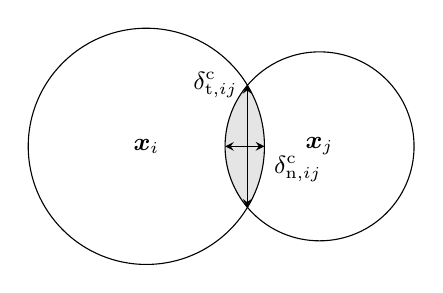
\begin{tikzpicture}
    \begin{scope}
        \clip  (0,0) circle(1.5);
        \filldraw[black!10]  (2.2,0) circle(1.2);
    \end{scope}
    \draw (0,0) circle(1.5) node {\small$\bm x_i$};
    \draw (2.2,0) circle(1.2) node {\small$\bm x_j$};
    
    \draw[<->,>=stealth,] (1,0)--(1.5,0) node[below right] {\small$\delta^\text{c}_{\text{n},ij}$};
    \draw[<->,>=stealth,] (1.28,-0.78)--(1.28,0.78) node[left] {\small$\delta^\text{c}_{\text{t},ij}$};
\end{tikzpicture}

\end{document}